\documentclass[11pt]{amsart}
\usepackage[margin=1.15in]{geometry}
\usepackage{amssymb,mathtools}
\usepackage{tikz,pgfplots}
\pgfplotsset{compat=1.18}
\usepackage[hidelinks]{hyperref}
\usepackage{booktabs}

\tikzset{
  gridline/.style={very thin,gray!35},
  stitch/.style={line width=0.9pt,black},
  loopfill/.style={fill=orange!30},
  lab/.style={font=\scriptsize,gray!80!black}
}

\newtheorem{theorem}{Theorem}[section]
\newtheorem{proposition}[theorem]{Proposition}
\newtheorem{lemma}[theorem]{Lemma}
\newtheorem{corollary}[theorem]{Corollary}
\theoremstyle{definition}
\newtheorem{definition}[theorem]{Definition}
\newtheorem{question}[theorem]{Question}
\theoremstyle{remark}
\newtheorem{remark}[theorem]{Remark}
\newtheorem{example}[theorem]{Example}

\newcommand{\Loops}{\operatorname{Loops}}
\newcommand{\E}{\mathbb{E}}
\newcommand{\ev}{\operatorname{ev}}
\newcommand{\od}{\operatorname{od}}
\newcommand{\U}{\mathsf{U}}
\newcommand{\D}{\mathsf{D}}

\title{The loop density of biased random hitomezashi patterns}
\author{Vamshi Jandhyala}
\address{London, United Kingdom}
\email{vamshi.jandhyala@gmail.com}
\subjclass[2020]{05A15, 05A19, 60K35, 68V20}
\keywords{hitomezashi, corner percolation, Dyck paths, continued fractions, loop density, Lean}
\date{Preprint v1, 22 November 2026}

\begin{document}

\begin{abstract}
A hitomezashi pattern is drawn by labelling every grid line $0$ or $1$ and stitching alternate unit
segments of each line, starting according to its label. Defant and Kravitz proved that when the labels
are fair coin flips, the expected number of closed loops in an $m\times n$ pattern is
$\bigl(\tfrac{\pi^2-9}{12}+o(1)\bigr)mn$. We compute the loop density when the labels are independent
and each is $0$ with probability $p$, for every $p\in(0,1)$:
\[
c(p)=2pq-\frac54+\frac{\pi^2p^2q^2}{6}\Bigl(2+\frac{3}{\sin^2\pi p}\Bigr)+\frac{\pi\,pq\,(1-3pq)\cot\pi p}{1-2p},
\qquad q=1-p,
\]
with the value $(\pi^2-9)/12$ at $p=\tfrac12$. The proof reads off the labels a loop forces from Pete's
pair of Dyck paths, which turns the density into a sum over weighted Dyck paths of fixed height. For
every $p$ the two-step transfer matrix of these weights has a double eigenvalue, the continuants
become linear functions of the index times powers of $pq$, and the sum reduces to Euler's partial fraction expansions
of $\cot$ and $\csc^2$. We prove that the fair coin uniquely minimises the density and give a
closed form for different biases on the two families of lines, with an explicit series truncation
bound. The label-counting lemmas, continuant identities and one-bias series evaluation are formalised
in Lean~4 with Mathlib.
\end{abstract}
\maketitle

\section{Introduction}

On every line of a square grid, stitch every other unit segment, and toss a coin for each line to decide whether
its stitching starts on the first segment or the second. The stitches close up into loops of many sizes. How many
loops per unit area does this produce, and how does the answer change when the coins are biased? For fair coins
Defant and Kravitz found the answer; this paper finds it for every bias.

Hitomezashi is a Japanese style of sashiko embroidery. To draw a pattern, give each vertical grid line
$x=i$ a label $\varepsilon_i\in\{0,1\}$ and each horizontal grid line $y=j$ a label $\eta_j\in\{0,1\}$.
On the line $x=i$, draw the unit segment from $(i,j)$ to $(i,j+1)$ exactly when $j\equiv\varepsilon_i
\pmod 2$; on the line $y=j$, draw the segment from $(i,j)$ to $(i+1,j)$ exactly when $i\equiv\eta_j
\pmod 2$. The drawn segments are the \emph{stitches}. Restricting to the rectangle $[0,n]\times[0,m]$,
with its $n+1$ vertical and $m+1$ horizontal lines labelled, gives an \emph{$m\times n$ hitomezashi
pattern}. These conventions are those of Defant and Kravitz~\cite{DK24}. Figure~\ref{fig:pattern} shows
an example.

In the infinite pattern every lattice point is an endpoint of exactly one vertical stitch and
exactly one horizontal stitch, because along each line the stitches alternate. In the finite pattern
the same holds at interior points, while a boundary point may meet fewer stitches. The stitches
therefore split into paths and closed curves, and the closed curves are the \emph{loops} of the
pattern. Write $\Loops(H)$ for the number of
loops of a pattern $H$, and $H_p(m,n)$ for the random $m\times n$ pattern whose $m+n+2$ labels are
independent, each equal to $0$ with probability $p$ and to $1$ with probability $q=1-p$.

\begin{figure}[t]
\centering
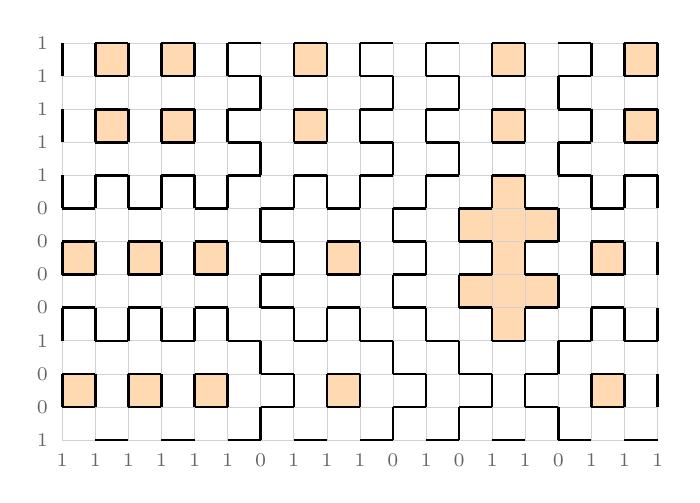
\begin{tikzpicture}[scale=0.42]
\fill[loopfill] (0,1) -- (0,2) -- (1,2) -- (1,1) -- cycle;
\fill[loopfill] (0,5) -- (0,6) -- (1,6) -- (1,5) -- cycle;
\fill[loopfill] (1,9) -- (1,10) -- (2,10) -- (2,9) -- cycle;
\fill[loopfill] (1,11) -- (1,12) -- (2,12) -- (2,11) -- cycle;
\fill[loopfill] (2,1) -- (2,2) -- (3,2) -- (3,1) -- cycle;
\fill[loopfill] (2,5) -- (2,6) -- (3,6) -- (3,5) -- cycle;
\fill[loopfill] (3,9) -- (3,10) -- (4,10) -- (4,9) -- cycle;
\fill[loopfill] (3,11) -- (3,12) -- (4,12) -- (4,11) -- cycle;
\fill[loopfill] (4,1) -- (4,2) -- (5,2) -- (5,1) -- cycle;
\fill[loopfill] (4,5) -- (4,6) -- (5,6) -- (5,5) -- cycle;
\fill[loopfill] (7,9) -- (7,10) -- (8,10) -- (8,9) -- cycle;
\fill[loopfill] (7,11) -- (7,12) -- (8,12) -- (8,11) -- cycle;
\fill[loopfill] (8,1) -- (8,2) -- (9,2) -- (9,1) -- cycle;
\fill[loopfill] (8,5) -- (8,6) -- (9,6) -- (9,5) -- cycle;
\fill[loopfill] (12,4) -- (12,5) -- (13,5) -- (13,6) -- (12,6) -- (12,7) -- (13,7) -- (13,8) -- (14,8) -- (14,7) -- (15,7) -- (15,6) -- (14,6) -- (14,5) -- (15,5) -- (15,4) -- (14,4) -- (14,3) -- (13,3) -- (13,4) -- cycle;
\fill[loopfill] (13,9) -- (13,10) -- (14,10) -- (14,9) -- cycle;
\fill[loopfill] (13,11) -- (13,12) -- (14,12) -- (14,11) -- cycle;
\fill[loopfill] (16,1) -- (16,2) -- (17,2) -- (17,1) -- cycle;
\fill[loopfill] (16,5) -- (16,6) -- (17,6) -- (17,5) -- cycle;
\fill[loopfill] (17,9) -- (17,10) -- (18,10) -- (18,9) -- cycle;
\fill[loopfill] (17,11) -- (17,12) -- (18,12) -- (18,11) -- cycle;
\draw[gridline] (0,0) grid (18,12);
\draw[stitch] (0,1) -- (0,2);
\draw[stitch] (0,3) -- (0,4);
\draw[stitch] (0,5) -- (0,6);
\draw[stitch] (0,7) -- (0,8);
\draw[stitch] (0,9) -- (0,10);
\draw[stitch] (0,11) -- (0,12);
\draw[stitch] (1,1) -- (1,2);
\draw[stitch] (1,3) -- (1,4);
\draw[stitch] (1,5) -- (1,6);
\draw[stitch] (1,7) -- (1,8);
\draw[stitch] (1,9) -- (1,10);
\draw[stitch] (1,11) -- (1,12);
\draw[stitch] (2,1) -- (2,2);
\draw[stitch] (2,3) -- (2,4);
\draw[stitch] (2,5) -- (2,6);
\draw[stitch] (2,7) -- (2,8);
\draw[stitch] (2,9) -- (2,10);
\draw[stitch] (2,11) -- (2,12);
\draw[stitch] (3,1) -- (3,2);
\draw[stitch] (3,3) -- (3,4);
\draw[stitch] (3,5) -- (3,6);
\draw[stitch] (3,7) -- (3,8);
\draw[stitch] (3,9) -- (3,10);
\draw[stitch] (3,11) -- (3,12);
\draw[stitch] (4,1) -- (4,2);
\draw[stitch] (4,3) -- (4,4);
\draw[stitch] (4,5) -- (4,6);
\draw[stitch] (4,7) -- (4,8);
\draw[stitch] (4,9) -- (4,10);
\draw[stitch] (4,11) -- (4,12);
\draw[stitch] (5,1) -- (5,2);
\draw[stitch] (5,3) -- (5,4);
\draw[stitch] (5,5) -- (5,6);
\draw[stitch] (5,7) -- (5,8);
\draw[stitch] (5,9) -- (5,10);
\draw[stitch] (5,11) -- (5,12);
\draw[stitch] (6,0) -- (6,1);
\draw[stitch] (6,2) -- (6,3);
\draw[stitch] (6,4) -- (6,5);
\draw[stitch] (6,6) -- (6,7);
\draw[stitch] (6,8) -- (6,9);
\draw[stitch] (6,10) -- (6,11);
\draw[stitch] (7,1) -- (7,2);
\draw[stitch] (7,3) -- (7,4);
\draw[stitch] (7,5) -- (7,6);
\draw[stitch] (7,7) -- (7,8);
\draw[stitch] (7,9) -- (7,10);
\draw[stitch] (7,11) -- (7,12);
\draw[stitch] (8,1) -- (8,2);
\draw[stitch] (8,3) -- (8,4);
\draw[stitch] (8,5) -- (8,6);
\draw[stitch] (8,7) -- (8,8);
\draw[stitch] (8,9) -- (8,10);
\draw[stitch] (8,11) -- (8,12);
\draw[stitch] (9,1) -- (9,2);
\draw[stitch] (9,3) -- (9,4);
\draw[stitch] (9,5) -- (9,6);
\draw[stitch] (9,7) -- (9,8);
\draw[stitch] (9,9) -- (9,10);
\draw[stitch] (9,11) -- (9,12);
\draw[stitch] (10,0) -- (10,1);
\draw[stitch] (10,2) -- (10,3);
\draw[stitch] (10,4) -- (10,5);
\draw[stitch] (10,6) -- (10,7);
\draw[stitch] (10,8) -- (10,9);
\draw[stitch] (10,10) -- (10,11);
\draw[stitch] (11,1) -- (11,2);
\draw[stitch] (11,3) -- (11,4);
\draw[stitch] (11,5) -- (11,6);
\draw[stitch] (11,7) -- (11,8);
\draw[stitch] (11,9) -- (11,10);
\draw[stitch] (11,11) -- (11,12);
\draw[stitch] (12,0) -- (12,1);
\draw[stitch] (12,2) -- (12,3);
\draw[stitch] (12,4) -- (12,5);
\draw[stitch] (12,6) -- (12,7);
\draw[stitch] (12,8) -- (12,9);
\draw[stitch] (12,10) -- (12,11);
\draw[stitch] (13,1) -- (13,2);
\draw[stitch] (13,3) -- (13,4);
\draw[stitch] (13,5) -- (13,6);
\draw[stitch] (13,7) -- (13,8);
\draw[stitch] (13,9) -- (13,10);
\draw[stitch] (13,11) -- (13,12);
\draw[stitch] (14,1) -- (14,2);
\draw[stitch] (14,3) -- (14,4);
\draw[stitch] (14,5) -- (14,6);
\draw[stitch] (14,7) -- (14,8);
\draw[stitch] (14,9) -- (14,10);
\draw[stitch] (14,11) -- (14,12);
\draw[stitch] (15,0) -- (15,1);
\draw[stitch] (15,2) -- (15,3);
\draw[stitch] (15,4) -- (15,5);
\draw[stitch] (15,6) -- (15,7);
\draw[stitch] (15,8) -- (15,9);
\draw[stitch] (15,10) -- (15,11);
\draw[stitch] (16,1) -- (16,2);
\draw[stitch] (16,3) -- (16,4);
\draw[stitch] (16,5) -- (16,6);
\draw[stitch] (16,7) -- (16,8);
\draw[stitch] (16,9) -- (16,10);
\draw[stitch] (16,11) -- (16,12);
\draw[stitch] (17,1) -- (17,2);
\draw[stitch] (17,3) -- (17,4);
\draw[stitch] (17,5) -- (17,6);
\draw[stitch] (17,7) -- (17,8);
\draw[stitch] (17,9) -- (17,10);
\draw[stitch] (17,11) -- (17,12);
\draw[stitch] (18,1) -- (18,2);
\draw[stitch] (18,3) -- (18,4);
\draw[stitch] (18,5) -- (18,6);
\draw[stitch] (18,7) -- (18,8);
\draw[stitch] (18,9) -- (18,10);
\draw[stitch] (18,11) -- (18,12);
\draw[stitch] (1,0) -- (2,0);
\draw[stitch] (3,0) -- (4,0);
\draw[stitch] (5,0) -- (6,0);
\draw[stitch] (7,0) -- (8,0);
\draw[stitch] (9,0) -- (10,0);
\draw[stitch] (11,0) -- (12,0);
\draw[stitch] (13,0) -- (14,0);
\draw[stitch] (15,0) -- (16,0);
\draw[stitch] (17,0) -- (18,0);
\draw[stitch] (0,1) -- (1,1);
\draw[stitch] (2,1) -- (3,1);
\draw[stitch] (4,1) -- (5,1);
\draw[stitch] (6,1) -- (7,1);
\draw[stitch] (8,1) -- (9,1);
\draw[stitch] (10,1) -- (11,1);
\draw[stitch] (12,1) -- (13,1);
\draw[stitch] (14,1) -- (15,1);
\draw[stitch] (16,1) -- (17,1);
\draw[stitch] (0,2) -- (1,2);
\draw[stitch] (2,2) -- (3,2);
\draw[stitch] (4,2) -- (5,2);
\draw[stitch] (6,2) -- (7,2);
\draw[stitch] (8,2) -- (9,2);
\draw[stitch] (10,2) -- (11,2);
\draw[stitch] (12,2) -- (13,2);
\draw[stitch] (14,2) -- (15,2);
\draw[stitch] (16,2) -- (17,2);
\draw[stitch] (1,3) -- (2,3);
\draw[stitch] (3,3) -- (4,3);
\draw[stitch] (5,3) -- (6,3);
\draw[stitch] (7,3) -- (8,3);
\draw[stitch] (9,3) -- (10,3);
\draw[stitch] (11,3) -- (12,3);
\draw[stitch] (13,3) -- (14,3);
\draw[stitch] (15,3) -- (16,3);
\draw[stitch] (17,3) -- (18,3);
\draw[stitch] (0,4) -- (1,4);
\draw[stitch] (2,4) -- (3,4);
\draw[stitch] (4,4) -- (5,4);
\draw[stitch] (6,4) -- (7,4);
\draw[stitch] (8,4) -- (9,4);
\draw[stitch] (10,4) -- (11,4);
\draw[stitch] (12,4) -- (13,4);
\draw[stitch] (14,4) -- (15,4);
\draw[stitch] (16,4) -- (17,4);
\draw[stitch] (0,5) -- (1,5);
\draw[stitch] (2,5) -- (3,5);
\draw[stitch] (4,5) -- (5,5);
\draw[stitch] (6,5) -- (7,5);
\draw[stitch] (8,5) -- (9,5);
\draw[stitch] (10,5) -- (11,5);
\draw[stitch] (12,5) -- (13,5);
\draw[stitch] (14,5) -- (15,5);
\draw[stitch] (16,5) -- (17,5);
\draw[stitch] (0,6) -- (1,6);
\draw[stitch] (2,6) -- (3,6);
\draw[stitch] (4,6) -- (5,6);
\draw[stitch] (6,6) -- (7,6);
\draw[stitch] (8,6) -- (9,6);
\draw[stitch] (10,6) -- (11,6);
\draw[stitch] (12,6) -- (13,6);
\draw[stitch] (14,6) -- (15,6);
\draw[stitch] (16,6) -- (17,6);
\draw[stitch] (0,7) -- (1,7);
\draw[stitch] (2,7) -- (3,7);
\draw[stitch] (4,7) -- (5,7);
\draw[stitch] (6,7) -- (7,7);
\draw[stitch] (8,7) -- (9,7);
\draw[stitch] (10,7) -- (11,7);
\draw[stitch] (12,7) -- (13,7);
\draw[stitch] (14,7) -- (15,7);
\draw[stitch] (16,7) -- (17,7);
\draw[stitch] (1,8) -- (2,8);
\draw[stitch] (3,8) -- (4,8);
\draw[stitch] (5,8) -- (6,8);
\draw[stitch] (7,8) -- (8,8);
\draw[stitch] (9,8) -- (10,8);
\draw[stitch] (11,8) -- (12,8);
\draw[stitch] (13,8) -- (14,8);
\draw[stitch] (15,8) -- (16,8);
\draw[stitch] (17,8) -- (18,8);
\draw[stitch] (1,9) -- (2,9);
\draw[stitch] (3,9) -- (4,9);
\draw[stitch] (5,9) -- (6,9);
\draw[stitch] (7,9) -- (8,9);
\draw[stitch] (9,9) -- (10,9);
\draw[stitch] (11,9) -- (12,9);
\draw[stitch] (13,9) -- (14,9);
\draw[stitch] (15,9) -- (16,9);
\draw[stitch] (17,9) -- (18,9);
\draw[stitch] (1,10) -- (2,10);
\draw[stitch] (3,10) -- (4,10);
\draw[stitch] (5,10) -- (6,10);
\draw[stitch] (7,10) -- (8,10);
\draw[stitch] (9,10) -- (10,10);
\draw[stitch] (11,10) -- (12,10);
\draw[stitch] (13,10) -- (14,10);
\draw[stitch] (15,10) -- (16,10);
\draw[stitch] (17,10) -- (18,10);
\draw[stitch] (1,11) -- (2,11);
\draw[stitch] (3,11) -- (4,11);
\draw[stitch] (5,11) -- (6,11);
\draw[stitch] (7,11) -- (8,11);
\draw[stitch] (9,11) -- (10,11);
\draw[stitch] (11,11) -- (12,11);
\draw[stitch] (13,11) -- (14,11);
\draw[stitch] (15,11) -- (16,11);
\draw[stitch] (17,11) -- (18,11);
\draw[stitch] (1,12) -- (2,12);
\draw[stitch] (3,12) -- (4,12);
\draw[stitch] (5,12) -- (6,12);
\draw[stitch] (7,12) -- (8,12);
\draw[stitch] (9,12) -- (10,12);
\draw[stitch] (11,12) -- (12,12);
\draw[stitch] (13,12) -- (14,12);
\draw[stitch] (15,12) -- (16,12);
\draw[stitch] (17,12) -- (18,12);
\node[lab] at (0,-0.6) {1};
\node[lab] at (1,-0.6) {1};
\node[lab] at (2,-0.6) {1};
\node[lab] at (3,-0.6) {1};
\node[lab] at (4,-0.6) {1};
\node[lab] at (5,-0.6) {1};
\node[lab] at (6,-0.6) {0};
\node[lab] at (7,-0.6) {1};
\node[lab] at (8,-0.6) {1};
\node[lab] at (9,-0.6) {1};
\node[lab] at (10,-0.6) {0};
\node[lab] at (11,-0.6) {1};
\node[lab] at (12,-0.6) {0};
\node[lab] at (13,-0.6) {1};
\node[lab] at (14,-0.6) {1};
\node[lab] at (15,-0.6) {0};
\node[lab] at (16,-0.6) {1};
\node[lab] at (17,-0.6) {1};
\node[lab] at (18,-0.6) {1};
\node[lab] at (-0.6,0) {1};
\node[lab] at (-0.6,1) {0};
\node[lab] at (-0.6,2) {0};
\node[lab] at (-0.6,3) {1};
\node[lab] at (-0.6,4) {0};
\node[lab] at (-0.6,5) {0};
\node[lab] at (-0.6,6) {0};
\node[lab] at (-0.6,7) {0};
\node[lab] at (-0.6,8) {1};
\node[lab] at (-0.6,9) {1};
\node[lab] at (-0.6,10) {1};
\node[lab] at (-0.6,11) {1};
\node[lab] at (-0.6,12) {1};
\end{tikzpicture}

\caption{A $12\times18$ pattern with labels drawn at $p=0.3$ (the labels are printed beside their
lines). Its $21$ loops are shaded. When $p$ is small the unit squares are the commonest loops.}
\label{fig:pattern}
\end{figure}

Defant and Kravitz~\cite[Theorem~1.6]{DK24} proved that
$\E[\Loops(H_{1/2}(m,n))]=\bigl(\tfrac{\pi^2-9}{12}+o(1)\bigr)mn$ as $\min\{m,n\}\to\infty$. Their
argument rests on a description, due to Pete~\cite{Pet08} in the language of corner percolation, of
every loop by a pair of Dyck paths of the same height. Pete also discussed independent biased labels;
Defant and Kravitz defined $H_p(m,n)$ for all $p$ but computed the density only in the fair case. This
note computes it for every bias.

\begin{theorem}\label{thm:main}
For every $p\in(0,1)$,
\[
\E[\Loops(H_p(m,n))]=(c(p)+o(1))\,mn\qquad(\min\{m,n\}\to\infty),
\]
where, for $p\neq\tfrac12$ and $q=1-p$,
\begin{equation}\label{eq:main}
c(p)=2pq-\frac54+\frac{\pi^2p^2q^2}{6}\Bigl(2+\frac{3}{\sin^2\pi p}\Bigr)
+\frac{\pi\,pq\,(1-3pq)\cot\pi p}{1-2p},
\end{equation}
and $c(\tfrac12)=(\pi^2-9)/12$, which is also the limit of~\eqref{eq:main} as $p\to\tfrac12$. The same
holds with loops replaced by the regions into which the stitches divide the rectangle.
\end{theorem}

The formula is symmetric under $p\leftrightarrow q$, as it must be. Translating a pattern by $(1,1)$
gives the pattern with labels $\varepsilon'_i=1-\varepsilon_{i-1}$ and $\eta'_j=1-\eta_{j-1}$; the labels
are independent and identically distributed, so the translated labels have the law of the
$q$-biased ones, and the loop density, which does not see a translation, is the same. The last term looks singular at $p=\tfrac12$, but
$\cot\pi p$ vanishes there to first order, and $\cot(\pi p)/(1-2p)\to\pi/2$. Substituting $p=\tfrac12$
into the remaining terms gives $-\tfrac34+\tfrac{5\pi^2}{96}+\tfrac{3\pi^2}{96}=\tfrac{\pi^2-9}{12}$.
Expanding~\eqref{eq:main} near $p=0$ and near $p=\tfrac12$, using the Laurent expansions of $\cot$ and
$\csc^2$ (we omit this computation), gives
\[
c(p)=\tfrac14-p+\tfrac{3+\pi^2}{6}\,p^2+O(p^3),\qquad
c(\tfrac12+\delta)=\tfrac{\pi^2-9}{12}+\tfrac{\pi^4-4\pi^2-48}{24}\,\delta^2+O(\delta^4).
\]
The value $\tfrac14$ at $p=0$ is the all-zero cloth, which is a grid of unit-square loops on a quarter
of the cells. The coefficient of $\delta^2$ is about $0.414$, so $p=\tfrac12$ is a strict local minimum.
Theorem~\ref{thm:monotone} proves that $c$ is strictly decreasing on $(0,\tfrac12]$ and hence, by
symmetry, that the fair coin is its unique global minimum (Figure~\ref{fig:density}).
Theorem~\ref{thm:two-bias} extends the density formula to distinct biases on the two families of lines.

\begin{figure}[t]
\centering
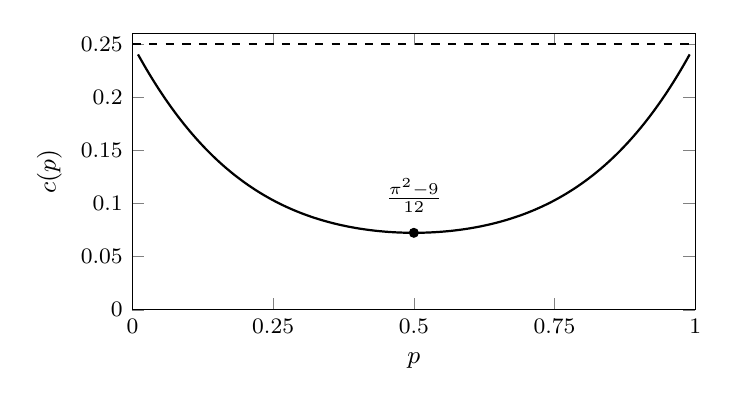
\begin{tikzpicture}
\begin{axis}[width=0.72\textwidth,height=0.42\textwidth,xmin=0,xmax=1,ymin=0,ymax=0.26,
  xlabel={$p$},ylabel={$c(p)$},xtick={0,0.25,0.5,0.75,1},ytick={0,0.05,0.1,0.15,0.2,0.25},
  tick label style={font=\footnotesize},yticklabel style={/pgf/number format/fixed,/pgf/number format/precision=2},label style={font=\small}]
\addplot[thick,smooth] coordinates {(0.010,0.240212) (0.015,0.235475) (0.020,0.230840) (0.025,0.226305) (0.030,0.221870) (0.035,0.217531) (0.040,0.213289) (0.045,0.209140) (0.050,0.205085) (0.055,0.201120) (0.060,0.197245) (0.065,0.193458) (0.070,0.189757) (0.075,0.186142) (0.080,0.182610) (0.085,0.179161) (0.090,0.175792) (0.095,0.172503) (0.100,0.169292) (0.105,0.166157) (0.110,0.163098) (0.115,0.160113) (0.120,0.157200) (0.125,0.154359) (0.130,0.151589) (0.135,0.148886) (0.140,0.146252) (0.145,0.143684) (0.150,0.141181) (0.155,0.138742) (0.160,0.136365) (0.165,0.134051) (0.170,0.131796) (0.175,0.129601) (0.180,0.127464) (0.185,0.125384) (0.190,0.123360) (0.195,0.121391) (0.200,0.119475) (0.205,0.117613) (0.210,0.115802) (0.215,0.114041) (0.220,0.112330) (0.225,0.110668) (0.230,0.109054) (0.235,0.107487) (0.240,0.105965) (0.245,0.104488) (0.250,0.103055) (0.255,0.101666) (0.260,0.100318) (0.265,0.099012) (0.270,0.097747) (0.275,0.096521) (0.280,0.095334) (0.285,0.094185) (0.290,0.093074) (0.295,0.091999) (0.300,0.090960) (0.305,0.089956) (0.310,0.088987) (0.315,0.088051) (0.320,0.087149) (0.325,0.086279) (0.330,0.085440) (0.335,0.084633) (0.340,0.083857) (0.345,0.083110) (0.350,0.082393) (0.355,0.081705) (0.360,0.081045) (0.365,0.080412) (0.370,0.079808) (0.375,0.079230) (0.380,0.078678) (0.385,0.078152) (0.390,0.077652) (0.395,0.077177) (0.400,0.076727) (0.405,0.076301) (0.410,0.075899) (0.415,0.075520) (0.420,0.075165) (0.425,0.074833) (0.430,0.074524) (0.435,0.074237) (0.440,0.073972) (0.445,0.073730) (0.450,0.073509) (0.455,0.073310) (0.460,0.073132) (0.465,0.072976) (0.470,0.072840) (0.475,0.072726) (0.480,0.072633) (0.485,0.072560) (0.490,0.072508) (0.495,0.072477) (0.500,0.072467) (0.505,0.072477) (0.510,0.072508) (0.515,0.072560) (0.520,0.072633) (0.525,0.072726) (0.530,0.072840) (0.535,0.072976) (0.540,0.073132) (0.545,0.073310) (0.550,0.073509) (0.555,0.073730) (0.560,0.073972) (0.565,0.074237) (0.570,0.074524) (0.575,0.074833) (0.580,0.075165) (0.585,0.075520) (0.590,0.075899) (0.595,0.076301) (0.600,0.076727) (0.605,0.077177) (0.610,0.077652) (0.615,0.078152) (0.620,0.078678) (0.625,0.079230) (0.630,0.079808) (0.635,0.080412) (0.640,0.081045) (0.645,0.081705) (0.650,0.082393) (0.655,0.083110) (0.660,0.083857) (0.665,0.084633) (0.670,0.085440) (0.675,0.086279) (0.680,0.087149) (0.685,0.088051) (0.690,0.088987) (0.695,0.089956) (0.700,0.090960) (0.705,0.091999) (0.710,0.093074) (0.715,0.094185) (0.720,0.095334) (0.725,0.096521) (0.730,0.097747) (0.735,0.099012) (0.740,0.100318) (0.745,0.101666) (0.750,0.103055) (0.755,0.104488) (0.760,0.105965) (0.765,0.107487) (0.770,0.109054) (0.775,0.110668) (0.780,0.112330) (0.785,0.114041) (0.790,0.115802) (0.795,0.117613) (0.800,0.119475) (0.805,0.121391) (0.810,0.123360) (0.815,0.125384) (0.820,0.127464) (0.825,0.129601) (0.830,0.131796) (0.835,0.134051) (0.840,0.136365) (0.845,0.138742) (0.850,0.141181) (0.855,0.143684) (0.860,0.146252) (0.865,0.148886) (0.870,0.151589) (0.875,0.154359) (0.880,0.157200) (0.885,0.160113) (0.890,0.163098) (0.895,0.166157) (0.900,0.169292) (0.905,0.172503) (0.910,0.175792) (0.915,0.179161) (0.920,0.182610) (0.925,0.186142) (0.930,0.189757) (0.935,0.193458) (0.940,0.197245) (0.945,0.201120) (0.950,0.205085) (0.955,0.209140) (0.960,0.213289) (0.965,0.217531) (0.970,0.221870) (0.975,0.226305) (0.980,0.230840) (0.985,0.235475) (0.990,0.240212)};
\addplot[only marks,mark=*,mark size=1.6pt] coordinates {(0.5,0.072467)};
\node[anchor=south,font=\footnotesize] at (axis cs:0.5,0.082) {$\frac{\pi^2-9}{12}$};
\addplot[dashed] coordinates {(0,0.25) (1,0.25)};
\end{axis}
\end{tikzpicture}

\caption{The loop density $c(p)$ of Theorem~\ref{thm:main}. The dashed line is the limit $\tfrac14$ at
$p\to0$ and $p\to1$; the dot is the value of Defant and Kravitz at $p=\tfrac12$.}
\label{fig:density}
\end{figure}

\subsection*{How the proof goes}
A fixed loop $L$ of width $w$ and height $h$ appears at a given position exactly when the $w+1$ vertical
and $h+1$ horizontal lines it uses carry the labels it needs, so its probability is a monomial in $p$
and $q$. Section~\ref{sec:labels} shows that the number of zeros the loop needs on its vertical lines
is determined by Pete's Dyck path: it is twice the number of up-steps that start at an odd height, plus
two, or twice the number that start at an even height, according to the parity of the position. So the
density becomes a sum over pairs of weighted Dyck paths of equal height
(Section~\ref{sec:series}), in which an up-step leaving an even level costs $q^2$ and one leaving an odd
level costs $p^2$. Flajolet's continued fraction theorem expresses the weight of the Dyck paths of height
exactly $k$ through continuants (Section~\ref{sec:dyck}). The coincidence that makes everything explicit
is that $(1-p^2-q^2)^2=4p^2q^2$ whenever $p+q=1$: the two-step transfer matrix has a double eigenvalue
for every $p$, the continuants are linear in the index times powers of $pq$, and the height-$k$ weights
decay like $k^{-2}$. The remaining series are partial fraction expansions of $\cot$ and $\csc^2$
(Section~\ref{sec:sum}).

\subsection*{Related work}
Pete~\cite{Pet08} studied the fair model as corner percolation and proved that all its components are
finite almost surely. In the ``Biased coins'' discussion of~\cite[Section~7]{Pet08}, he also considered
independent biased labels, as here, and observed that his finiteness proof extends to every
$p\in(0,1)$. Marchand, Marcovici and Siest~\cite{MMS25} studied a biased corner percolation in which the
\emph{orientations} of the lines, which are the labels added to the line index modulo~$2$, are
independent and biased; there infinite paths appear (see also Siest's thesis~\cite{Sie24}). Under
independent biased labels, as here, the orientations alternate in bias from one line to the next, so
the two models differ. Defant, Kravitz and Tenner~\cite{DKT23}, Ren and Zhang~\cite{RZ25} and
Xie~\cite{Xie25} studied hitomezashi patterns on other surfaces and other extensions, and
Wildstrom~\cite{Wil24} studied the depth of nested regions in uniformly random patterns. None of these
computes a loop density away from $p=\tfrac12$. Pete's remark fits the mechanism found here: the double
eigenvalue of Lemma~\ref{lem:Q} is the weighted-path counterpart of his observation that alternately
biased walks behave like simple random walks.

\subsection*{Formalisation}
The label-counting lemmas of Section~\ref{sec:labels}, the continuant identities of
Section~\ref{sec:dyck} and the series evaluation of Section~\ref{sec:sum}, including both cases of the
density formula, are proved in Lean~4 with Mathlib~\cite{Mathlib}. The correspondence with loops and
the passage from loop probabilities to the limiting density use the cited results and the paper
proofs. Section~\ref{sec:checks} gives the precise scope of the formalisation and the computational
checks.

\section{The labels a loop forces}\label{sec:labels}

\subsection{Walking along a loop}
Because each lattice point meets one vertical and one horizontal stitch, a walk along stitches
alternates vertical and horizontal steps.

\begin{lemma}\label{lem:walk}
Let $z_0,z_1,\dots,z_L$ be a walk along stitches whose steps alternate, the step from $z_t$ to
$z_{t+1}$ being vertical for even $t$ and horizontal for odd $t$. Put
$\sigma\equiv x(z_0)+y(z_0)\pmod 2$. If $t$ is even and $z_t=(i,j)$, then
\[
\varepsilon_i\equiv\begin{cases}\sigma+i&\text{if the step goes up,}\\ \sigma+i+1&\text{if it goes down.}\end{cases}
\]
If $t$ is odd and $z_t=(i,j)$, then $\eta_j\equiv\sigma+1+j$ if the step goes right and
$\eta_j\equiv\sigma+j$ if it goes left. All congruences are modulo $2$.
\end{lemma}

\begin{proof}
Each step changes $x+y$ by $\pm1$, so $x(z_t)+y(z_t)\equiv\sigma+t$. Let $t$ be even, so $i+j\equiv\sigma$.
An upward step from $(i,j)$ uses the stitch from $(i,j)$ to $(i,j+1)$, which exists exactly when
$\varepsilon_i\equiv j\equiv\sigma+i$. A downward step uses the stitch from $(i,j-1)$ to $(i,j)$, so
$\varepsilon_i\equiv j-1\equiv\sigma+i+1$. For odd $t$ we have $i+j\equiv\sigma+1$; a step to the right
needs $\eta_j\equiv i\equiv\sigma+1+j$, and a step to the left needs $\eta_j\equiv i-1\equiv\sigma+j$.
\end{proof}

In particular, all the vertical stitches of a loop on one vertical line are traversed in the same
direction, and likewise for horizontal lines; this is \cite[Lemma~2.3]{DK24}.

\subsection{Pete's Dyck paths}
Let $L$ be a loop whose bounding box is $[x_0,x_0+w]\times[y_0,y_0+h]$. Since its steps alternate, $L$
has vertical stitches on every line $x=x_0+t$ ($0\le t\le w$) and horizontal stitches on every line
$y=y_0+t$ ($0\le t\le h$). Orient $L$ counterclockwise. The \emph{vertical word} of $L$ (Figure~\ref{fig:mechanism}) is
$V(L)=s_0s_1\cdots s_w$, where $s_t=\U$ if the stitches of $L$ on $x=x_0+t$ run south and $s_t=\D$ if
they run north. The \emph{horizontal word} $H(L)$ records $\U$ for the lines $y=y_0+t$ on which $L$ runs
east and $\D$ for those on which it runs west. On the westernmost line a counterclockwise loop runs
south, and on the southernmost line it runs east, so both words begin with $\U$ and end with $\D$.

\begin{theorem}[Pete~{\cite{Pet08}}; see {\cite[Theorem~3.1]{DK24}}]\label{thm:pete}
Every loop has odd width and odd height. Its words have the form $V(L)=\U P\D$ and $H(L)=\U P'\D$ where
$P$ and $P'$ are Dyck paths of semilengths $(w-1)/2$ and $(h-1)/2$ and of the same height. The map
$L\mapsto(P,P')$ is a bijection from loops modulo translation onto pairs of Dyck paths of equal height.
\end{theorem}

We record the words with the convention that makes the outer steps $\U$ and $\D$. We checked this
reading against every loop of every labelling of the $7\times7$ grid (Section~\ref{sec:checks}).

\subsection{Counting the zeros}
For a word $P$ in $\U,\D$ starting at height $0$, write $\ev(P)$ and $\od(P)$ for the numbers of
up-steps of $P$ that start at an even and at an odd height.

\begin{lemma}\label{lem:zeros}
Let $L$ be a loop with vertical word $\U P\D$, and put $A=1+\od(P)$ and $B=\ev(P)$. Among the labels
$\varepsilon_{x_0},\dots,\varepsilon_{x_0+w}$ of the lines $L$ uses, the number of zeros is $2A$ or
$2B$, and the number of ones is the other. The same holds for the horizontal labels with $P'$ in place
of $P$.
\end{lemma}

\begin{proof}
Write $\U P\D=s_0\cdots s_w$. A southward step is a downward step, so by Lemma~\ref{lem:walk}, applied
to $L$ walked from a point where it is about to take a vertical step,
$\varepsilon_{x_0+t}\equiv[s_t=\U]+t+\kappa$ for a constant $\kappa$. Hence $\varepsilon_{x_0+t}=0$
exactly when $[s_t=\U]\equiv t+\kappa$.

Let $h_t$ be the height of the word $s_0\cdots s_w$ before step $t$, so $h_t\equiv t$. If $\kappa\equiv
0$, a zero occurs at an up-step from an odd height or a down-step from an even height. The potential
$\phi(h)=\lfloor h/2\rfloor$ rises by one at an up-step from an odd height, falls by one at a down-step
from an even height, and is unchanged at every other step. The word returns to height $0$, so these two
kinds of step are equally many, and the number of zeros is twice the number of up-steps from an odd
height. If $\kappa\equiv1$, the same argument with $\lceil h/2\rceil$ shows that the number of zeros is
twice the number of up-steps from an even height. In $\U P\D$ the first step starts at height $0$ and
the up-steps of $P$ start one level higher than in $P$. Thus its numbers of up-steps from odd and even
heights are $\ev(P)=B$ and $1+\od(P)=A$, respectively: the zero count is $2B$ when $\kappa\equiv0$
and $2A$ when $\kappa\equiv1$. The ones are the remaining $w+1-2B=2A$ or $w+1-2A=2B$ labels,
since $w+1=2(A+B)$. The
horizontal case is identical, because by Lemma~\ref{lem:walk} the horizontal labels are also of the
form $[\,\text{step}=\U\,]+t+\kappa'$.
\end{proof}

\begin{figure}[t]
\centering
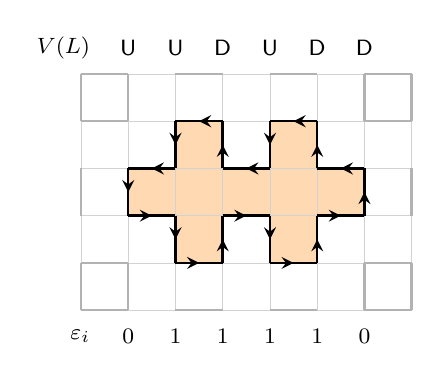
\begin{tikzpicture}[scale=0.6]
\fill[loopfill] (2,2) -- (2,1) -- (3,1) -- (3,2) -- (4,2) -- (4,1) -- (5,1) -- (5,2) -- (6,2) -- (6,3) -- (5,3) -- (5,4) -- (4,4) -- (4,3) -- (3,3) -- (3,4) -- (2,4) -- (2,3) -- (1,3) -- (1,2) -- cycle;
\draw[gridline] (0,0) grid (7,5);
\draw[stitch,gray!60] (0,0) -- (0,1);
\draw[stitch,gray!60] (0,2) -- (0,3);
\draw[stitch,gray!60] (0,4) -- (0,5);
\draw[stitch,gray!60] (1,0) -- (1,1);
\draw[stitch,gray!60] (1,2) -- (1,3);
\draw[stitch,gray!60] (1,4) -- (1,5);
\draw[stitch,gray!60] (2,1) -- (2,2);
\draw[stitch,gray!60] (2,3) -- (2,4);
\draw[stitch,gray!60] (3,1) -- (3,2);
\draw[stitch,gray!60] (3,3) -- (3,4);
\draw[stitch,gray!60] (4,1) -- (4,2);
\draw[stitch,gray!60] (4,3) -- (4,4);
\draw[stitch,gray!60] (5,1) -- (5,2);
\draw[stitch,gray!60] (5,3) -- (5,4);
\draw[stitch,gray!60] (6,0) -- (6,1);
\draw[stitch,gray!60] (6,2) -- (6,3);
\draw[stitch,gray!60] (6,4) -- (6,5);
\draw[stitch,gray!60] (7,0) -- (7,1);
\draw[stitch,gray!60] (7,2) -- (7,3);
\draw[stitch,gray!60] (7,4) -- (7,5);
\draw[stitch,gray!60] (0,0) -- (1,0);
\draw[stitch,gray!60] (2,0) -- (3,0);
\draw[stitch,gray!60] (4,0) -- (5,0);
\draw[stitch,gray!60] (6,0) -- (7,0);
\draw[stitch,gray!60] (0,1) -- (1,1);
\draw[stitch,gray!60] (2,1) -- (3,1);
\draw[stitch,gray!60] (4,1) -- (5,1);
\draw[stitch,gray!60] (6,1) -- (7,1);
\draw[stitch,gray!60] (1,2) -- (2,2);
\draw[stitch,gray!60] (3,2) -- (4,2);
\draw[stitch,gray!60] (5,2) -- (6,2);
\draw[stitch,gray!60] (1,3) -- (2,3);
\draw[stitch,gray!60] (3,3) -- (4,3);
\draw[stitch,gray!60] (5,3) -- (6,3);
\draw[stitch,gray!60] (0,4) -- (1,4);
\draw[stitch,gray!60] (2,4) -- (3,4);
\draw[stitch,gray!60] (4,4) -- (5,4);
\draw[stitch,gray!60] (6,4) -- (7,4);
\draw[stitch,gray!60] (0,5) -- (1,5);
\draw[stitch,gray!60] (2,5) -- (3,5);
\draw[stitch,gray!60] (4,5) -- (5,5);
\draw[stitch,gray!60] (6,5) -- (7,5);
\draw[stitch,->,>=stealth] (2,2) -- (2.0,1.5);
\draw[stitch] (2,2) -- (2,1);
\draw[stitch,->,>=stealth] (2,1) -- (2.5,1.0);
\draw[stitch] (2,1) -- (3,1);
\draw[stitch,->,>=stealth] (3,1) -- (3.0,1.5);
\draw[stitch] (3,1) -- (3,2);
\draw[stitch,->,>=stealth] (3,2) -- (3.5,2.0);
\draw[stitch] (3,2) -- (4,2);
\draw[stitch,->,>=stealth] (4,2) -- (4.0,1.5);
\draw[stitch] (4,2) -- (4,1);
\draw[stitch,->,>=stealth] (4,1) -- (4.5,1.0);
\draw[stitch] (4,1) -- (5,1);
\draw[stitch,->,>=stealth] (5,1) -- (5.0,1.5);
\draw[stitch] (5,1) -- (5,2);
\draw[stitch,->,>=stealth] (5,2) -- (5.5,2.0);
\draw[stitch] (5,2) -- (6,2);
\draw[stitch,->,>=stealth] (6,2) -- (6.0,2.5);
\draw[stitch] (6,2) -- (6,3);
\draw[stitch,->,>=stealth] (6,3) -- (5.5,3.0);
\draw[stitch] (6,3) -- (5,3);
\draw[stitch,->,>=stealth] (5,3) -- (5.0,3.5);
\draw[stitch] (5,3) -- (5,4);
\draw[stitch,->,>=stealth] (5,4) -- (4.5,4.0);
\draw[stitch] (5,4) -- (4,4);
\draw[stitch,->,>=stealth] (4,4) -- (4.0,3.5);
\draw[stitch] (4,4) -- (4,3);
\draw[stitch,->,>=stealth] (4,3) -- (3.5,3.0);
\draw[stitch] (4,3) -- (3,3);
\draw[stitch,->,>=stealth] (3,3) -- (3.0,3.5);
\draw[stitch] (3,3) -- (3,4);
\draw[stitch,->,>=stealth] (3,4) -- (2.5,4.0);
\draw[stitch] (3,4) -- (2,4);
\draw[stitch,->,>=stealth] (2,4) -- (2.0,3.5);
\draw[stitch] (2,4) -- (2,3);
\draw[stitch,->,>=stealth] (2,3) -- (1.5,3.0);
\draw[stitch] (2,3) -- (1,3);
\draw[stitch,->,>=stealth] (1,3) -- (1.0,2.5);
\draw[stitch] (1,3) -- (1,2);
\draw[stitch,->,>=stealth] (1,2) -- (1.5,2.0);
\draw[stitch] (1,2) -- (2,2);
\node[font=\footnotesize] at (1,5.55) {$\mathsf{U}$};
\node[font=\footnotesize] at (1,-0.55) {$0$};
\node[font=\footnotesize] at (2,5.55) {$\mathsf{U}$};
\node[font=\footnotesize] at (2,-0.55) {$1$};
\node[font=\footnotesize] at (3,5.55) {$\mathsf{D}$};
\node[font=\footnotesize] at (3,-0.55) {$1$};
\node[font=\footnotesize] at (4,5.55) {$\mathsf{U}$};
\node[font=\footnotesize] at (4,-0.55) {$1$};
\node[font=\footnotesize] at (5,5.55) {$\mathsf{D}$};
\node[font=\footnotesize] at (5,-0.55) {$1$};
\node[font=\footnotesize] at (6,5.55) {$\mathsf{D}$};
\node[font=\footnotesize] at (6,-0.55) {$0$};
\node[font=\footnotesize,anchor=east] at (0.4,5.55) {$V(L)$};
\node[font=\footnotesize,anchor=east] at (0.4,-0.55) {$\varepsilon_i$};
\end{tikzpicture}

\caption{A loop $L$ of width $5$ and height $3$, oriented counterclockwise, with the other stitches in grey. Above
each vertical line is its letter in $V(L)=\U\,\U\D\U\D\,\D$ ($\U$ where $L$ runs south), below it the line's
label. Here $P=\U\D\U\D$; both its up-steps start at height $0$, so $\od(P)=0$, $\ev(P)=2$, $A=1$ and $B=2$. As
Lemma~\ref{lem:zeros} says, the six vertical lines carry $2A=2$ zeros and $2B=4$ ones.}\label{fig:mechanism}
\end{figure}

\begin{example}
Figure~\ref{fig:mechanism} shows the lemma on a loop of width $5$. The smallest loop is the unit square: $P$ is empty, $A=1$, $B=0$, and its two vertical lines must both
be labelled $0$ or both $1$, according to position. The next one, of width and height $3$, has
$P=P'=\U\D$, so $A=B=1$: each of its two families of four lines needs two zeros and two ones (for
instance the labels $1,0,0,1$).
\end{example}

\begin{corollary}\label{cor:prob}
Let $L$ be a loop with words $\U P\D$, $\U P'\D$, constants $A,B$ from $P$ and $A',B'$ from $P'$, and
put $u=p^2$, $v=q^2$. Among the four translates $L+(a,b)$ with $a,b\in\{0,1\}$, the probability that
the translate is a loop of the random pattern (when its box lies in the rectangle) averages to
\[
\bar\omega(L)=\tfrac14\bigl(u^Av^B+u^Bv^A\bigr)\bigl(u^{A'}v^{B'}+u^{B'}v^{A'}\bigr).
\]
\end{corollary}

\begin{proof}
A translate of $L$ is a loop of the pattern exactly when every stitch of it is present: each of its
lines carries one of its stitches, which fixes that line's label, and once all its stitches are present
each of its points already has its two stitches, so nothing else can join it. These $w+h+2$ lines are
distinct and their labels are independent, so the probability is $p^{z}q^{w+h+2-z}$, where $z$ is the
number of zeros required. Shifting the walk of Lemma~\ref{lem:walk} by $(1,0)$ adds $1$ to $\sigma$
and to every line index $i$, so the vertical labels are unchanged while every horizontal label is
complemented; shifting by $(0,1)$ complements the vertical labels and leaves the horizontal ones. By
Lemma~\ref{lem:zeros} the four translates therefore realise each of the four combinations of
$\{2A,2B\}$ zeros on the vertical lines with $\{2A',2B'\}$ on the horizontal lines exactly once.
\end{proof}

\section{From loops to a series}\label{sec:series}

For $k\ge0$ let $\mathcal D_k$ be the set of Dyck paths of height exactly $k$ (the empty path has height
$0$), and define
\begin{equation}\label{eq:X}
X_k(p)=\sum_{P\in\mathcal D_k}\Bigl(u^{1+\od(P)}v^{\ev(P)}+v^{1+\od(P)}u^{\ev(P)}\Bigr),
\qquad u=p^2,\ v=q^2.
\end{equation}
By Theorem~\ref{thm:pete} and Corollary~\ref{cor:prob},
\begin{equation}\label{eq:c}
\sum_{L}\bar\omega(L)=\frac14\sum_{k\ge0}X_k(p)^2,
\end{equation}
the sum on the left running over loops modulo translation; all terms are non-negative, so the
rearrangement is free. Section~\ref{sec:sum} shows that the right-hand side is finite and equals the
expression of Theorem~\ref{thm:main}. We first check that it is the density.

\begin{proposition}\label{prop:density}
Let $c(p)=\frac14\sum_kX_k(p)^2<\infty$. Then $\E[\Loops(H_p(m,n))]=(c(p)+o(1))mn$.
\end{proposition}

\begin{proof}
This is the argument of \cite[Lemma~6.1]{DK24}, adjusted for the dependence on position. A loop $L$ of
width $w\le n$ and height $h\le m$ has $(n+1-w)(m+1-h)$ translates whose boxes lie in the rectangle. For
$\alpha\in\{0,1\}$, the number of $a\in\{0,\dots,M\}$ with $a\equiv\alpha$ lies between
$\lfloor(M+1)/2\rfloor$ and $\lceil(M+1)/2\rceil$. Since $w,h\ge1$, each parity class of positions
contains at most $\tfrac{n+1}{2}\cdot\tfrac{m+1}{2}$ translates, so by Corollary~\ref{cor:prob}
\[
\E[\Loops(H_p(m,n))]\le(n+1)(m+1)\sum_L\bar\omega(L)=(n+1)(m+1)\,c(p).
\]
Conversely, if $w,h\le r$ then each parity class contains at least $\tfrac{n-r}{2}\cdot\tfrac{m-r}{2}$
translates, so $\E[\Loops(H_p(m,n))]\ge(n-r)(m-r)\sum_{w,h\le r}\bar\omega(L)$. Divide by $mn$, let
$m,n\to\infty$ and then $r\to\infty$.
\end{proof}

The number of regions is the number of loops plus the number of regions touching the boundary of the
rectangle, which is at most $2(m+n)$ \cite[Section~6]{DK24}; so Theorem~\ref{thm:main} for regions
follows from the theorem for loops.

\section{Weighted Dyck paths of fixed height}\label{sec:dyck}

Give each up-step of a Dyck path that starts at level $i$ the weight $a_i\ge0$, and each down-step the
weight $1$; the weight of a path is the product of the weights of its steps. Define the continuants
\[
Q_0=Q_1=1,\quad Q_{h+2}=Q_{h+1}-a_hQ_h,\qquad P_0=0,\ P_1=1,\quad P_{h+2}=P_{h+1}-a_hP_h.
\]

\begin{proposition}[Flajolet~{\cite{Fla80}}; {\cite[Proposition~V.3(ii)]{FS09}}]\label{prop:cf}
As formal power series in $z$, with each $a_i$ replaced by $a_iz$, the generating function of Dyck
paths of height at most $k$ is $P_{k+1}/Q_{k+1}$.
\end{proposition}

\begin{lemma}\label{lem:eval}
If $Q_j(1)>0$ for every $j\le k+1$, then the total weight of the Dyck paths of height at most $k$ is
finite and equals $P_{k+1}(1)/Q_{k+1}(1)$.
\end{lemma}

\begin{proof}
Let $\rho_j(z)=Q_{j+1}(z)/Q_j(z)$, so $\rho_0=1$ and $\rho_j=1-za_{j-1}/\rho_{j-1}$. By induction on
$j$, each $\rho_j$ is positive and non-increasing on $[0,1]$: if $\rho_{j-1}$ is, then
$za_{j-1}/\rho_{j-1}$ is non-decreasing, so $\rho_j$ is non-increasing and
$\rho_j(z)\ge\rho_j(1)=Q_{j+1}(1)/Q_j(1)>0$. Hence $Q_{k+1}$ has no zero in $[0,1]$. The series of
Proposition~\ref{prop:cf} has non-negative coefficients; by Pringsheim's theorem
\cite[Theorem~IV.6]{FS09} its radius of convergence $R$ is a singularity of the function it defines.
That function is the rational function $P_{k+1}/Q_{k+1}$, which is analytic on a neighbourhood of
$[0,1]$, so $R>1$ and the series converges at $z=1$ to $P_{k+1}(1)/Q_{k+1}(1)$.
\end{proof}

\begin{lemma}\label{lem:casoratian}
$P_{h+1}Q_h-P_hQ_{h+1}=a_0a_1\cdots a_{h-1}$. Consequently, under the hypothesis of
Lemma~\ref{lem:eval}, the total weight of the Dyck paths of height exactly $k$ is
\[
\frac{P_{k+1}}{Q_{k+1}}-\frac{P_k}{Q_k}=\frac{a_0a_1\cdots a_{k-1}}{Q_kQ_{k+1}}.
\]
\end{lemma}

\begin{proof}
At $h=0$ both sides equal $1$, and the recurrences give
$P_{h+2}Q_{h+1}-P_{h+1}Q_{h+2}=a_h(P_{h+1}Q_h-P_hQ_{h+1})$.
\end{proof}

In~\eqref{eq:X}, the term $u^{1+\od(P)}v^{\ev(P)}$ is $u$ times the weight of $P$ for the alternating
weights $a_i=v$ ($i$ even), $a_i=u$ ($i$ odd), and the other term is $v$ times the weight for the
alternating weights with $u$ and $v$ exchanged.

\begin{lemma}\label{lem:Q}
Let $p+q=1$, $r=pq\ne0$, and $a_i=q^2$ for even $i$, $a_i=p^2$ for odd $i$. Then for all $j\ge0$
\[
Q_{2j+1}=(j+1)\,r^j,\qquad r\,Q_{2j}=r^j\,p\,(j+q).
\]
\end{lemma}

\begin{proof}
Both hold at $j=0$. If they hold at $j$, then $rQ_{2j+2}=r(j+1)r^j-q^2r^jp(j+q)=r^{j+1}p(j+1+q)$, using
$1-q=p$; and then $rQ_{2j+3}=r^{j+1}p(j+1+q)-p^2(j+1)r^{j+1}=r^{j+2}(j+2)$, using $1-p=q$.
\end{proof}

The lemma is where the double eigenvalue shows. The two-step recurrence for alternating weights $s,t$
has characteristic polynomial $\mu^2-(1-s-t)\mu+st$, whose discriminant $(1-s-t)^2-4st$ vanishes
identically when $s=q^2$, $t=p^2$ and $p+q=1$. In general it vanishes exactly when
$\sqrt s+\sqrt t=1$ or $\lvert\sqrt s-\sqrt t\rvert=1$, so our weights lie on the boundary of the
subcritical region $\sqrt s+\sqrt t<1$. Inside that region the two roots are distinct and the
height-$k$ weights behave geometrically in $k$; on the boundary the double root makes the
continuants linear in the index times powers of $pq$ instead.

\begin{proposition}\label{prop:X}
For $0<p<1$ and $j\ge0$,
\[
X_{2j}(p)=\frac{r}{j+1}\Bigl(\frac{p}{j+q}+\frac{q}{j+p}\Bigr),\qquad
X_{2j+1}(p)=\frac{r}{j+1}\Bigl(\frac{q}{j+1+q}+\frac{p}{j+1+p}\Bigr).
\]
\end{proposition}

\begin{proof}
By Lemma~\ref{lem:Q} and its image under $p\leftrightarrow q$, all continuants are positive, so
Lemmas~\ref{lem:eval} and~\ref{lem:casoratian} apply. For $k=2j$ the product of weights is $(pq)^{2j}$,
and $Q_{2j}Q_{2j+1}=r^{2j-1}p(j+q)(j+1)$, so the first family contributes
$u\cdot r/(p(j+q)(j+1))=r\,p/((j+q)(j+1))$; the second gives the same with $p$ and $q$ exchanged.
For $k=2j+1$ the product is $r^{2j}q^2$ and $Q_{2j+1}Q_{2j+2}=(j+1)r^{2j}p(j+1+q)$, giving
$u\,q^2/((j+1)p(j+1+q))=r\,q/((j+1)(j+1+q))$, and again the same with $p,q$ exchanged.
\end{proof}

So $X_k(p)\sim 4pq/k^2$ for large $k$, whatever $p$ is. At $p=\tfrac12$ the two weight families
coincide, $X_k(\tfrac12)=\tfrac12F_k(\tfrac14)$ in the notation of \cite[Section~6]{DK24}, and the
proposition recovers the values that Defant and Kravitz obtain from a formula of Kreweras.

\section{Summing the series}\label{sec:sum}

Three classical series are needed, each for $0<x<1$:
\begin{align}
\sum_{n\ge1}\frac1{n^2}&=\frac{\pi^2}6,\label{eq:zeta}\\
\sum_{n\ge1}\frac{2}{n^2-x^2}&=\frac1x\Bigl(\frac1x-\pi\cot\pi x\Bigr),\label{eq:K}\\
\sum_{n\ge1}\Bigl(\frac1{(n+x)^2}+\frac1{(n-x)^2}\Bigr)&=\frac{\pi^2}{\sin^2\pi x}-\frac1{x^2}.\label{eq:T}
\end{align}
The first is Euler's. The second is Euler's partial fraction expansion
$\pi\cot\pi x=\frac1x+\sum_{n\ge1}\bigl(\frac1{x-n}+\frac1{x+n}\bigr)$, rearranged; Mathlib contains both
\cite{Mathlib}. The third is the derivative of the second: on $(0,b)$ with $b=\frac{1+x}2<1$ the
derivatives $-(y-n)^{-2}-(y+n)^{-2}$ of the terms are bounded by $\bigl((1-b)^{-2}+1\bigr)n^{-2}$, so the
expansion may be differentiated term by term, and $\frac{d}{dy}(\pi\cot\pi y-\frac1y)=
-\pi^2/\sin^2\pi y+1/y^2$.

\begin{proof}[Proof of Theorem~\ref{thm:main}]
By Proposition~\ref{prop:density} it suffices to evaluate $c(p)=\frac14\sum_kX_k(p)^2$. Group the terms
in pairs $k=2j,2j+1$ and put $n=j+1$. Proposition~\ref{prop:X} reads
\[
X_{2j}=\frac rn\Bigl(\frac p{n-p}+\frac q{n-q}\Bigr),\qquad X_{2j+1}=\frac rn\Bigl(\frac q{n+q}+\frac p{n+p}\Bigr),
\]
and for $p\ne q$ partial fractions give
\begin{multline*}
\frac{X_{2j}^2+X_{2j+1}^2}4=\frac{r^2}4\Bigl[\frac8{n^2}+T_n(p)+T_n(q)
-\Bigl(4+\frac{2p}{q-p}\Bigr)K_n(p)-\Bigl(4-\frac{2q}{q-p}\Bigr)K_n(q)\Bigr],
\end{multline*}
with $T_n(x)=(n+x)^{-2}+(n-x)^{-2}$ and $K_n(x)=2/(n^2-x^2)$. Read in words: the squares of the
simple fractions produce the $T_n$, the cross terms with $1/n$ and with each other produce the $K_n$,
and nothing else appears. Every series converges, both halves of each pair are non-negative, and
\eqref{eq:zeta}, \eqref{eq:K} and \eqref{eq:T} sum the bracket. With $\sin\pi q=\sin\pi p$ and $\cot\pi q=-\cot\pi p$
the result is
\[
\frac{r^2}4\Bigl[\frac{4\pi^2}3+\frac{2\pi^2}{\sin^2\pi p}-\frac1{p^2}-\frac1{q^2}
-\Bigl(4+\frac{2p}{q-p}\Bigr)\frac{1-\pi p\cot\pi p}{p^2}
-\Bigl(4-\frac{2q}{q-p}\Bigr)\frac{1+\pi q\cot\pi p}{q^2}\Bigr],
\]
which simplifies to~\eqref{eq:main}. For $p=q=\tfrac12$ the same grouping gives
$\frac1{64}\bigl[8n^{-2}+4T_n(\tfrac12)-8K_n(\tfrac12)\bigr]$, whose sum is
$\frac1{64}\bigl[\tfrac{4\pi^2}{3}+4(\pi^2-4)-32\bigr]=\tfrac{\pi^2-9}{12}$.
\end{proof}

\section{Consequences and extensions}\label{sec:extensions}

\subsection{The fair coin uniquely minimises the density}

\begin{theorem}\label{thm:monotone}
The density $c(p)$ is strictly decreasing on $(0,\tfrac12]$ and strictly increasing on
$[\tfrac12,1)$. In particular,
\[
\frac{\pi^2-9}{12}\le c(p)<\frac14,
\]
with equality on the left only at $p=\tfrac12$. More quantitatively, for
$\delta=p-\tfrac12$,
\begin{equation}\label{eq:stability}
c(p)-c(\tfrac12)\ge\frac{12-\pi^2}{6}\,\delta^2
  +\frac{\pi^2-6}{3}\,\delta^4.
\end{equation}
\end{theorem}

\begin{proof}
Put $s=(1-2p)^2$ and $F(s)=c((1-\sqrt{s})/2)$ for $0\le s<1$. We will show that $F'(s)>0$.
The odd-denominator forms of the cotangent and cosecant identities of Section~\ref{sec:sum} are
\[
\frac{\tan(\pi t/2)}{t}=\frac4\pi\sum_{\substack{\ell\ge1\\\ell\text{ odd}}}
 \frac1{\ell^2-t^2},\qquad
\sec^2(\pi t/2)=\frac8{\pi^2}\sum_{\substack{\ell\ge1\\\ell\text{ odd}}}
 \frac{\ell^2+t^2}{(\ell^2-t^2)^2}.
\]
The first follows by subtracting the even-denominator terms from~\eqref{eq:K}; differentiating
$t$ times the first gives the second. Both extend continuously to $t=0$.
Substitute these identities into~\eqref{eq:main}, with $t=1-2p$ and $s=t^2$, and separate
the term $\ell=1$. The result is
\begin{equation}\label{eq:monotone-series}
F(s)=-\frac14+\frac{s}{2}+\frac{\pi^2(1-s)^2}{48}
 +\frac12\sum_{\substack{\ell\ge3\\\ell\text{ odd}}} f_{\ell^2}(s),\qquad
f_A(s)=\frac{(1-s)\bigl(A(1+s)-2s^2\bigr)}{(A-s)^2}.
\end{equation}
For $A\ge9$ and $0\le s\le1$, direct differentiation gives
\[
f_A'(s)+\frac{2s}{A-1}
=\frac{2(1-s)\bigl(A(A-2)+A(1-s)(1+2s)+s^3\bigr)}{(A-1)(A-s)^3}\ge0.
\]
The summands in~\eqref{eq:monotone-series} and their derivatives are $O(\ell^{-2})$ uniformly
on $[0,1]$, so termwise differentiation is valid. Since
\[
\sum_{\substack{\ell\ge3\\\ell\text{ odd}}}\frac1{\ell^2-1}
=\frac14\sum_{j\ge1}\frac1{j(j+1)}=\frac14,
\]
we obtain
\begin{equation}\label{eq:derivative-bound}
F'(s)\ge\frac12-\frac{\pi^2(1-s)}{24}-\frac{s}{4}
=\frac{12-\pi^2}{24}(1-s)+\frac{s}{4}>0.
\end{equation}
Symmetry now gives the asserted monotonicity, and the endpoint limit $1/4$ gives the upper
bound. Integrating~\eqref{eq:derivative-bound} from $0$ to $s=4\delta^2$ yields
\eqref{eq:stability}.
\end{proof}

\subsection{Different biases on the two families of lines}

Let $H_{p_1,p_2}(m,n)$ have independent labels, with a vertical label equal to $0$ with
probability $p_1$ and a horizontal label equal to $0$ with probability $p_2$. The following
closed form includes coincident and complementary biases without singular denominators.
Write $\operatorname{sinc}(z)=\sin z/z$ for $z\ne0$, with $\operatorname{sinc}(0)=1$.
For $0<x,y<1$, define
\[
U(x)=\frac1x\Bigl(\frac1x-\pi\cot\pi x\Bigr),\qquad
V(x,y)=\frac{\pi^2\operatorname{sinc}(\pi(y-x))}{\sin\pi x\,\sin\pi y}-\frac1{xy}.
\]
In particular, $V(x,x)=\pi^2/\sin^2\pi x-1/x^2$.

\begin{theorem}\label{thm:two-bias}
For $p_1,p_2\in(0,1)$, put $q_i=1-p_i$, $r_i=p_iq_i$, $(a_0,a_1)=(p_1,q_1)$ and
$(b_0,b_1)=(p_2,q_2)$. Then
\[
\E[\Loops(H_{p_1,p_2}(m,n))]=(c(p_1,p_2)+o(1))mn,
\]
where
\begin{equation}\label{eq:two-bias}
c(p_1,p_2)=\frac{r_1r_2}{4}\left[\frac{4\pi^2}{3}
 -2\sum_{i=0}^1\bigl(U(a_i)+U(b_i)\bigr)
 +\sum_{i,j=0}^1V(a_i,b_j)\right].
\end{equation}
The same density holds for regions. If
\[
c_N(p_1,p_2)=\frac14\sum_{j=0}^N\bigl(X_{2j}(p_1)X_{2j}(p_2)
 +X_{2j+1}(p_1)X_{2j+1}(p_2)\bigr),
\]
then, for every integer $N\ge1$,
\begin{equation}\label{eq:tail}
0\le c(p_1,p_2)-c_N(p_1,p_2)\le\frac{r_1r_2}{6N^3}\le\frac1{96N^3}.
\end{equation}
In particular, this gives a uniform truncation bound for the one-bias density when $p_1=p_2$.
\end{theorem}

\begin{proof}
Corollary~\ref{cor:prob} becomes a product of a vertical and a horizontal weight. The bounds
below prove convergence, so the proof of Proposition~\ref{prop:density} gives
\[
c(p_1,p_2)=\frac14\sum_{k\ge0}X_k(p_1)X_k(p_2).
\]
For $m\in\mathbb Z\setminus\{0\}$ put
\[
A_p(m)=\frac2m-\frac1{m+p}-\frac1{m+(1-p)}.
\]
Proposition~\ref{prop:X} gives $X_{2j}(p)=p(1-p)A_p(-j-1)$ and
$X_{2j+1}(p)=p(1-p)A_p(j+1)$. Therefore
\[
c(p_1,p_2)=\frac{r_1r_2}{4}\sum_{m\ne0}A_{p_1}(m)A_{p_2}(m).
\]
Expanding the product, every resulting series is absolutely convergent. The identities of
Section~\ref{sec:sum}, with positive and negative indices paired, give
\[
\sum_{m\ne0}\frac1{m^2}=\frac{\pi^2}{3},\qquad
\sum_{m\ne0}\frac1{m(m+x)}=U(x),\qquad
\sum_{m\ne0}\frac1{(m+x)(m+y)}=V(x,y).
\]
For the last identity when $x\ne y$, partial fractions and the cotangent expansion give
$(G(x)-G(y))/(y-x)$, where $G(x)=\pi\cot\pi x-1/x$.
The identity $\cot\pi x-\cot\pi y=\sin\pi(y-x)/(\sin\pi x\sin\pi y)$ gives $V(x,y)$.
When $x=y$, use~\eqref{eq:T}. Substitution proves~\eqref{eq:two-bias}.

For $j\ge1$, Proposition~\ref{prop:X} also gives
\[
0<X_{2j}(p)\le\frac{p(1-p)}{j(j+1)},\qquad
0<X_{2j+1}(p)\le\frac{p(1-p)}{(j+1)^2}.
\]
These estimates prove convergence and, using $\sum_{j>N}j^{-4}\le\int_N^\infty x^{-4}\,dx$,
give
\[
0\le c(p_1,p_2)-c_N(p_1,p_2)
\le\frac{r_1r_2}{2}\sum_{j>N}\frac1{j^4}
\le\frac{r_1r_2}{6N^3}.
\]
The uniform bound follows from $r_i\le1/4$. The boundary-region estimate of
Section~\ref{sec:series} gives the assertion for regions.
\end{proof}

\begin{remark}
Pete~\cite[Section~7, ``Biased coins'']{Pet08} observes that with independent $p$-biased labels his
height-function walks have alternating biases, and that his proof that all components of the infinite
pattern are finite almost surely goes through verbatim for every $p\in(0,1)$. This
differs from the biased-orientation model of~\cite{MMS25}, which has infinite paths almost surely.
\end{remark}

\begin{question}
Pete~\cite[Section~7]{Pet08} asks whether his exponent for the expected length of a typical cycle
survives the bias: the main coefficients of his estimates are unchanged, and the open point is
whether the cancellation of the leading term in his equation~(5.20) still happens for biased labels. Does the explicit form of Proposition~\ref{prop:X} settle it?
Simulations suggest that the exponent does not depend on $p$. We traced every loop in $200$ random
$12000\times12000$ patterns at each of $p=0.5,0.4,0.3,0.2,0.15$. The local slope of
$\log\E[\text{length}\mid\text{diameter}]$ against $\log(\text{diameter})$, over diameters from
$250$ to $1000$, lies between $1.26$ and $1.30$ for every $p$. Pete's value is
$(\sqrt{17}+1)/4=1.2808$. The simulation, its fixed seeds and the histograms are in the
accompanying data (\texttt{verify/exponent\_sim}).
\end{question}

\begin{question}
What is the asymptotic order of $\operatorname{Var}\Loops(H_p(m,n))$, and under what
normalisation, if any, does the loop count satisfy a central limit theorem? The labels of a whole line are shared by every loop that uses it, so the loop counts of
distant parts of the pattern are correlated.
\end{question}

\section{Verification and formalisation}\label{sec:checks}

\begin{table}[h]
\centering\footnotesize
\begin{tabular}{@{}p{0.33\textwidth}p{0.25\textwidth}p{0.36\textwidth}@{}}
\toprule
Statement & Status & Where\\
\midrule
Lemma~\ref{lem:walk} & formalised & \texttt{Parity.lean}\\
Theorem~\ref{thm:pete} & cited \cite{Pet08,DK24}; reading checked & \texttt{verify/per\_loop.py}\\
Lemma~\ref{lem:zeros} & formalised & \texttt{LabelWord.lean}: \texttt{label\_word}\\
Corollary~\ref{cor:prob}, Proposition~\ref{prop:density} & proved here, not formalised & checked by \texttt{verify/monte\_carlo.py}\\
Proposition~\ref{prop:cf} & cited \cite{Fla80,FS09} & \\
Lemma~\ref{lem:eval} & proved here, not formalised & \\
Lemmas~\ref{lem:casoratian},~\ref{lem:Q}, Proposition~\ref{prop:X} & formalised & \texttt{Continuant.lean}\\
\eqref{eq:K}, \eqref{eq:T}, Section~\ref{sec:sum} & formalised & \texttt{Series.lean}: \texttt{hasSum\_density}\\
Theorems~\ref{thm:monotone},~\ref{thm:two-bias} & proved here, not formalised & \texttt{verify/extensions.py}\\
\bottomrule
\end{tabular}
\end{table}

The Lean files prove, for $0<p<1$ and $p\ne\tfrac12$, that $\sum_k X_k(p)^2/4$ converges to the right
side of~\eqref{eq:main}, and that at $p=\tfrac12$ it converges to $(\pi^2-9)/12$, with $X_k$ defined
from the continuants as in Lemma~\ref{lem:casoratian}. They use only the standard axioms; a mutation
suite of fifteen planted errors in the statements, among them each constant of~\eqref{eq:main}, is
rejected in full.

Four independent scripts check the loop correspondence and the density computations. The first
enumerates every labelling of the $7\times7$ grid and, for each of the $209{,}579$ loop occurrences,
checks that its words have the form $\U P\D$ with Dyck paths of equal height and that the labels it
uses have the zero counts of Lemma~\ref{lem:zeros}. The second sums~\eqref{eq:X} directly over Dyck paths
of height up to $59$ and semilength up to $1500$, and also sums Proposition~\ref{prop:X} to $25$ digits,
and compares both with~\eqref{eq:main} at $p=0.1,0.3,0.45,0.7$. The third samples $300$ random
$200\times200$ patterns at $p=0.3$ and $p=0.15$ and compares the mean loop count with the exact
finite-size expectation from the proof of Proposition~\ref{prop:density}. The fourth checks the
two-bias density of Theorem~\ref{thm:two-bias} against its closed form. A fifth script,
\texttt{verify/extensions.py}, checks the rational derivative identity used in
Theorem~\ref{thm:monotone}, the two-bias formula at coincident and complementary biases, and the
truncation intervals of~\eqref{eq:tail}. The additional results of Section~\ref{sec:extensions} have
paper proofs and are not formalised in Lean.

\subsection*{Declaration}
During the preparation of this work the author used Claude (Anthropic; model Claude Opus~5.5, via Claude
Code) and Codex (OpenAI; codex-cli 0.163.0, model gpt-6.1-sol). Claude originated the reduction to weighted
Dyck paths, the evaluation of the density series, the Lean formalisation and the verification programs, and
drafted the text. Codex corrected the proof of Lemma~\ref{lem:zeros}, originated Theorem~\ref{thm:monotone}
and the truncation bound of Theorem~\ref{thm:two-bias}, searched the literature and refereed the manuscript
and code. Claude rechecked each of Codex's contributions, and the computations are confirmed by the
formal proofs and independent programs described above. The author chose the problem, directed the work and takes full
responsibility for the content. This first version is released before the author's own line-by-line
reading of the text.

\subsection*{Data availability}
{\sloppy The verification scripts, the Lean source with pinned Lean and Mathlib dependencies and the build
instructions are archived with this preprint at \url{https://doi.org/10.5281/zenodo.24448300}. The same files
are in the folder \texttt{biased-hitomezashi-loops} of \url{https://github.com/jvvk/mathematics}, at tag
\texttt{biased-hitomezashi-loops-v1}. The correspondence between the paper and the Lean proofs is documented
in \texttt{lean/README.md}.\par}

\begin{thebibliography}{99}

\bibitem{DK24} C.~Defant and N.~Kravitz, Loops and regions in Hitomezashi patterns,
\emph{Discrete Math.} \textbf{347} (2024), 113693. \url{https://doi.org/10.1016/j.disc.2023.113693}

\bibitem{DKT23} C.~Defant, N.~Kravitz and B.~E.~Tenner, Extensions of hitomezashi patterns,
\emph{Discrete Math.} \textbf{346} (2023), 113555. \url{https://doi.org/10.1016/j.disc.2023.113555}

\bibitem{Fla80} P.~Flajolet, Combinatorial aspects of continued fractions, \emph{Discrete Math.}
\textbf{32} (1980), 125--161. \url{https://doi.org/10.1016/0012-365X(80)90050-3}

\bibitem{FS09} P.~Flajolet and R.~Sedgewick, \emph{Analytic Combinatorics}, Cambridge University Press,
Cambridge, 2009.

\bibitem{MMS25} R.~Marchand, I.~Marcovici and P.~Siest, Corner percolation with preferential directions,
\emph{ALEA Lat. Am. J. Probab. Math. Stat.} \textbf{22} (2025), 233--244.
\url{https://doi.org/10.30757/ALEA.v22-09}

\bibitem{Mathlib} The mathlib Community, The Lean mathematical library, in \emph{Proceedings of the 9th
ACM SIGPLAN International Conference on Certified Programs and Proofs (CPP 2020)}, ACM, 2020, 367--381.
\url{https://doi.org/10.1145/3372885.3373824}

\bibitem{Pet08} G.~Pete, Corner percolation on $\mathbb Z^2$ and the square root of $17$, \emph{Ann.
Probab.} \textbf{36} (2008), 1711--1747. \url{https://doi.org/10.1214/07-AOP373}

\bibitem{Sie24} P.~Siest, \emph{\'Etude d'un mod\`ele de percolation avec contrainte, et de mod\`eles
\`a croissance al\'eatoire lin\'eaire}, PhD thesis, Universit\'e de Lorraine, 2024.
\url{https://hal.univ-lorraine.fr/tel-04996092}

\bibitem{RZ25} Q.~Ren and S.~Zhang, Toroidal hitomezashi patterns, \emph{Discrete Math.} \textbf{348}
(2025), 114231. \url{https://doi.org/10.1016/j.disc.2024.114231}

\bibitem{Wil24} D.~J.~Wildstrom, Enclave depth in hitomezashi stitchery, in \emph{Proceedings of Bridges
2024: Mathematics, Art, Music, Architecture, Culture}, 2024, 357--360.
\url{https://archive.bridgesmathart.org/2024/bridges2024-357.html}

\bibitem{Xie25} E.~Xie, Cylindrical hitomezashi patterns, preprint (2025), arXiv:2509.04880.

\end{thebibliography}
\end{document}
